% Generated by Sphinx.
\def\sphinxdocclass{report}
\documentclass[letterpaper,10pt,english]{sphinxmanual}
\usepackage[utf8]{inputenc}
\DeclareUnicodeCharacter{00A0}{\nobreakspace}
\usepackage{cmap}
\usepackage[T1]{fontenc}
\usepackage{babel}
\usepackage{times}
\usepackage[Bjarne]{fncychap}
\usepackage{longtable}
\usepackage{sphinx}
\usepackage{multirow}


\title{AIMBAT Documentation}
\date{May 22, 2014}
\release{0.1.2}
\author{Lay Kuan Loh, Xiaoting Lou, \& Suzan van der Lee}
\newcommand{\sphinxlogo}{}
\renewcommand{\releasename}{Release}
\makeindex

\makeatletter
\def\PYG@reset{\let\PYG@it=\relax \let\PYG@bf=\relax%
    \let\PYG@ul=\relax \let\PYG@tc=\relax%
    \let\PYG@bc=\relax \let\PYG@ff=\relax}
\def\PYG@tok#1{\csname PYG@tok@#1\endcsname}
\def\PYG@toks#1+{\ifx\relax#1\empty\else%
    \PYG@tok{#1}\expandafter\PYG@toks\fi}
\def\PYG@do#1{\PYG@bc{\PYG@tc{\PYG@ul{%
    \PYG@it{\PYG@bf{\PYG@ff{#1}}}}}}}
\def\PYG#1#2{\PYG@reset\PYG@toks#1+\relax+\PYG@do{#2}}

\expandafter\def\csname PYG@tok@gd\endcsname{\def\PYG@tc##1{\textcolor[rgb]{0.63,0.00,0.00}{##1}}}
\expandafter\def\csname PYG@tok@gu\endcsname{\let\PYG@bf=\textbf\def\PYG@tc##1{\textcolor[rgb]{0.50,0.00,0.50}{##1}}}
\expandafter\def\csname PYG@tok@gt\endcsname{\def\PYG@tc##1{\textcolor[rgb]{0.00,0.27,0.87}{##1}}}
\expandafter\def\csname PYG@tok@gs\endcsname{\let\PYG@bf=\textbf}
\expandafter\def\csname PYG@tok@gr\endcsname{\def\PYG@tc##1{\textcolor[rgb]{1.00,0.00,0.00}{##1}}}
\expandafter\def\csname PYG@tok@cm\endcsname{\let\PYG@it=\textit\def\PYG@tc##1{\textcolor[rgb]{0.25,0.50,0.56}{##1}}}
\expandafter\def\csname PYG@tok@vg\endcsname{\def\PYG@tc##1{\textcolor[rgb]{0.73,0.38,0.84}{##1}}}
\expandafter\def\csname PYG@tok@m\endcsname{\def\PYG@tc##1{\textcolor[rgb]{0.13,0.50,0.31}{##1}}}
\expandafter\def\csname PYG@tok@mh\endcsname{\def\PYG@tc##1{\textcolor[rgb]{0.13,0.50,0.31}{##1}}}
\expandafter\def\csname PYG@tok@cs\endcsname{\def\PYG@tc##1{\textcolor[rgb]{0.25,0.50,0.56}{##1}}\def\PYG@bc##1{\setlength{\fboxsep}{0pt}\colorbox[rgb]{1.00,0.94,0.94}{\strut ##1}}}
\expandafter\def\csname PYG@tok@ge\endcsname{\let\PYG@it=\textit}
\expandafter\def\csname PYG@tok@vc\endcsname{\def\PYG@tc##1{\textcolor[rgb]{0.73,0.38,0.84}{##1}}}
\expandafter\def\csname PYG@tok@il\endcsname{\def\PYG@tc##1{\textcolor[rgb]{0.13,0.50,0.31}{##1}}}
\expandafter\def\csname PYG@tok@go\endcsname{\def\PYG@tc##1{\textcolor[rgb]{0.20,0.20,0.20}{##1}}}
\expandafter\def\csname PYG@tok@cp\endcsname{\def\PYG@tc##1{\textcolor[rgb]{0.00,0.44,0.13}{##1}}}
\expandafter\def\csname PYG@tok@gi\endcsname{\def\PYG@tc##1{\textcolor[rgb]{0.00,0.63,0.00}{##1}}}
\expandafter\def\csname PYG@tok@gh\endcsname{\let\PYG@bf=\textbf\def\PYG@tc##1{\textcolor[rgb]{0.00,0.00,0.50}{##1}}}
\expandafter\def\csname PYG@tok@ni\endcsname{\let\PYG@bf=\textbf\def\PYG@tc##1{\textcolor[rgb]{0.84,0.33,0.22}{##1}}}
\expandafter\def\csname PYG@tok@nl\endcsname{\let\PYG@bf=\textbf\def\PYG@tc##1{\textcolor[rgb]{0.00,0.13,0.44}{##1}}}
\expandafter\def\csname PYG@tok@nn\endcsname{\let\PYG@bf=\textbf\def\PYG@tc##1{\textcolor[rgb]{0.05,0.52,0.71}{##1}}}
\expandafter\def\csname PYG@tok@no\endcsname{\def\PYG@tc##1{\textcolor[rgb]{0.38,0.68,0.84}{##1}}}
\expandafter\def\csname PYG@tok@na\endcsname{\def\PYG@tc##1{\textcolor[rgb]{0.25,0.44,0.63}{##1}}}
\expandafter\def\csname PYG@tok@nb\endcsname{\def\PYG@tc##1{\textcolor[rgb]{0.00,0.44,0.13}{##1}}}
\expandafter\def\csname PYG@tok@nc\endcsname{\let\PYG@bf=\textbf\def\PYG@tc##1{\textcolor[rgb]{0.05,0.52,0.71}{##1}}}
\expandafter\def\csname PYG@tok@nd\endcsname{\let\PYG@bf=\textbf\def\PYG@tc##1{\textcolor[rgb]{0.33,0.33,0.33}{##1}}}
\expandafter\def\csname PYG@tok@ne\endcsname{\def\PYG@tc##1{\textcolor[rgb]{0.00,0.44,0.13}{##1}}}
\expandafter\def\csname PYG@tok@nf\endcsname{\def\PYG@tc##1{\textcolor[rgb]{0.02,0.16,0.49}{##1}}}
\expandafter\def\csname PYG@tok@si\endcsname{\let\PYG@it=\textit\def\PYG@tc##1{\textcolor[rgb]{0.44,0.63,0.82}{##1}}}
\expandafter\def\csname PYG@tok@s2\endcsname{\def\PYG@tc##1{\textcolor[rgb]{0.25,0.44,0.63}{##1}}}
\expandafter\def\csname PYG@tok@vi\endcsname{\def\PYG@tc##1{\textcolor[rgb]{0.73,0.38,0.84}{##1}}}
\expandafter\def\csname PYG@tok@nt\endcsname{\let\PYG@bf=\textbf\def\PYG@tc##1{\textcolor[rgb]{0.02,0.16,0.45}{##1}}}
\expandafter\def\csname PYG@tok@nv\endcsname{\def\PYG@tc##1{\textcolor[rgb]{0.73,0.38,0.84}{##1}}}
\expandafter\def\csname PYG@tok@s1\endcsname{\def\PYG@tc##1{\textcolor[rgb]{0.25,0.44,0.63}{##1}}}
\expandafter\def\csname PYG@tok@gp\endcsname{\let\PYG@bf=\textbf\def\PYG@tc##1{\textcolor[rgb]{0.78,0.36,0.04}{##1}}}
\expandafter\def\csname PYG@tok@sh\endcsname{\def\PYG@tc##1{\textcolor[rgb]{0.25,0.44,0.63}{##1}}}
\expandafter\def\csname PYG@tok@ow\endcsname{\let\PYG@bf=\textbf\def\PYG@tc##1{\textcolor[rgb]{0.00,0.44,0.13}{##1}}}
\expandafter\def\csname PYG@tok@sx\endcsname{\def\PYG@tc##1{\textcolor[rgb]{0.78,0.36,0.04}{##1}}}
\expandafter\def\csname PYG@tok@bp\endcsname{\def\PYG@tc##1{\textcolor[rgb]{0.00,0.44,0.13}{##1}}}
\expandafter\def\csname PYG@tok@c1\endcsname{\let\PYG@it=\textit\def\PYG@tc##1{\textcolor[rgb]{0.25,0.50,0.56}{##1}}}
\expandafter\def\csname PYG@tok@kc\endcsname{\let\PYG@bf=\textbf\def\PYG@tc##1{\textcolor[rgb]{0.00,0.44,0.13}{##1}}}
\expandafter\def\csname PYG@tok@c\endcsname{\let\PYG@it=\textit\def\PYG@tc##1{\textcolor[rgb]{0.25,0.50,0.56}{##1}}}
\expandafter\def\csname PYG@tok@mf\endcsname{\def\PYG@tc##1{\textcolor[rgb]{0.13,0.50,0.31}{##1}}}
\expandafter\def\csname PYG@tok@err\endcsname{\def\PYG@bc##1{\setlength{\fboxsep}{0pt}\fcolorbox[rgb]{1.00,0.00,0.00}{1,1,1}{\strut ##1}}}
\expandafter\def\csname PYG@tok@kd\endcsname{\let\PYG@bf=\textbf\def\PYG@tc##1{\textcolor[rgb]{0.00,0.44,0.13}{##1}}}
\expandafter\def\csname PYG@tok@ss\endcsname{\def\PYG@tc##1{\textcolor[rgb]{0.32,0.47,0.09}{##1}}}
\expandafter\def\csname PYG@tok@sr\endcsname{\def\PYG@tc##1{\textcolor[rgb]{0.14,0.33,0.53}{##1}}}
\expandafter\def\csname PYG@tok@mo\endcsname{\def\PYG@tc##1{\textcolor[rgb]{0.13,0.50,0.31}{##1}}}
\expandafter\def\csname PYG@tok@mi\endcsname{\def\PYG@tc##1{\textcolor[rgb]{0.13,0.50,0.31}{##1}}}
\expandafter\def\csname PYG@tok@kn\endcsname{\let\PYG@bf=\textbf\def\PYG@tc##1{\textcolor[rgb]{0.00,0.44,0.13}{##1}}}
\expandafter\def\csname PYG@tok@o\endcsname{\def\PYG@tc##1{\textcolor[rgb]{0.40,0.40,0.40}{##1}}}
\expandafter\def\csname PYG@tok@kr\endcsname{\let\PYG@bf=\textbf\def\PYG@tc##1{\textcolor[rgb]{0.00,0.44,0.13}{##1}}}
\expandafter\def\csname PYG@tok@s\endcsname{\def\PYG@tc##1{\textcolor[rgb]{0.25,0.44,0.63}{##1}}}
\expandafter\def\csname PYG@tok@kp\endcsname{\def\PYG@tc##1{\textcolor[rgb]{0.00,0.44,0.13}{##1}}}
\expandafter\def\csname PYG@tok@w\endcsname{\def\PYG@tc##1{\textcolor[rgb]{0.73,0.73,0.73}{##1}}}
\expandafter\def\csname PYG@tok@kt\endcsname{\def\PYG@tc##1{\textcolor[rgb]{0.56,0.13,0.00}{##1}}}
\expandafter\def\csname PYG@tok@sc\endcsname{\def\PYG@tc##1{\textcolor[rgb]{0.25,0.44,0.63}{##1}}}
\expandafter\def\csname PYG@tok@sb\endcsname{\def\PYG@tc##1{\textcolor[rgb]{0.25,0.44,0.63}{##1}}}
\expandafter\def\csname PYG@tok@k\endcsname{\let\PYG@bf=\textbf\def\PYG@tc##1{\textcolor[rgb]{0.00,0.44,0.13}{##1}}}
\expandafter\def\csname PYG@tok@se\endcsname{\let\PYG@bf=\textbf\def\PYG@tc##1{\textcolor[rgb]{0.25,0.44,0.63}{##1}}}
\expandafter\def\csname PYG@tok@sd\endcsname{\let\PYG@it=\textit\def\PYG@tc##1{\textcolor[rgb]{0.25,0.44,0.63}{##1}}}

\def\PYGZbs{\char`\\}
\def\PYGZus{\char`\_}
\def\PYGZob{\char`\{}
\def\PYGZcb{\char`\}}
\def\PYGZca{\char`\^}
\def\PYGZam{\char`\&}
\def\PYGZlt{\char`\<}
\def\PYGZgt{\char`\>}
\def\PYGZsh{\char`\#}
\def\PYGZpc{\char`\%}
\def\PYGZdl{\char`\$}
\def\PYGZhy{\char`\-}
\def\PYGZsq{\char`\'}
\def\PYGZdq{\char`\"}
\def\PYGZti{\char`\~}
% for compatibility with earlier versions
\def\PYGZat{@}
\def\PYGZlb{[}
\def\PYGZrb{]}
\makeatother

\begin{document}

\maketitle
\tableofcontents
\phantomsection\label{index::doc}


Contents:


\chapter{Introduction}
\label{docfiles/introduction:introduction}\label{docfiles/introduction:welcome-to-aimbat-s-documentation}\label{docfiles/introduction::doc}
AIMBAT (Automated and Interactive Measurement of Body wave Arrival Times) is an open-source software package for efficiently measuring teleseismic body wave arrival times for large seismic arrays {\hyperref[docfiles/citations:louvanderleelloyd2013-seismologicalresearchletters]{{[}LouVanderleeLloyd2013-SeismologicalResearchLetters{]}}}. It is based on a widely used method called MCCC (Multi-Channel Cross-Correlation) {\hyperref[docfiles/citations:vandecarcrosson1990-bulletinseismologicalsocietyofamerica]{{[}VandecarCrosson1990-BulletinSeismologicalSocietyOfAmerica{]}}}. The package is automated in the sense of initially aligning seismograms for MCCC which is achieved by an ICCS (Iterative Cross Correlation and Stack) algorithm. Meanwhile, a GUI (graphical user interface) is built to perform seismogram quality control interactively. Therefore, user processing time is reduced while valuable input from a user's expertise is retained. As a byproduct, SAC {\hyperref[docfiles/citations:goldsteindodgefirpo2003-internationalgeophysics]{{[}GoldsteinDodgeFirpo2003-InternationalGeophysics{]}}} plotting and phase picking functionalities are replicated and enhanced.

Modules and scripts included in the AIMBAT package were developed using \href{http://www.python.org/}{Python programming language} and its open-source modules on the Mac OS X platform since 2009. The original MCCC {\hyperref[docfiles/citations:vandecarcrosson1990-bulletinseismologicalsocietyofamerica]{{[}VandecarCrosson1990-BulletinSeismologicalSocietyOfAmerica{]}}} code was transcribed into Python. The GUI of AIMBAT was inspired and initiated at the \href{http://www.iris.edu/hq/es\_course/content/2009.html}{2009 EarthScope USArray Data Processing and Analysis Short Course}. AIMBAT runs on Mac OS X, Linux/Unix and Windows thanks to the platform-independent feature of Python.
It has been tested on Mac OS 10.6.8 and 10.7 and Fedora 16.

The AIMBAT software package is distributed under the \href{http://www.gnu.org/licenses/gpl.html}{GNU General Public License Version 3 (GPLv3)} as published by the Free Software Foundation.


\chapter{Installation}
\label{docfiles/installing:installation}\label{docfiles/installing::doc}

\section{Getting your operating system}
\label{docfiles/installing:getting-your-operating-system}
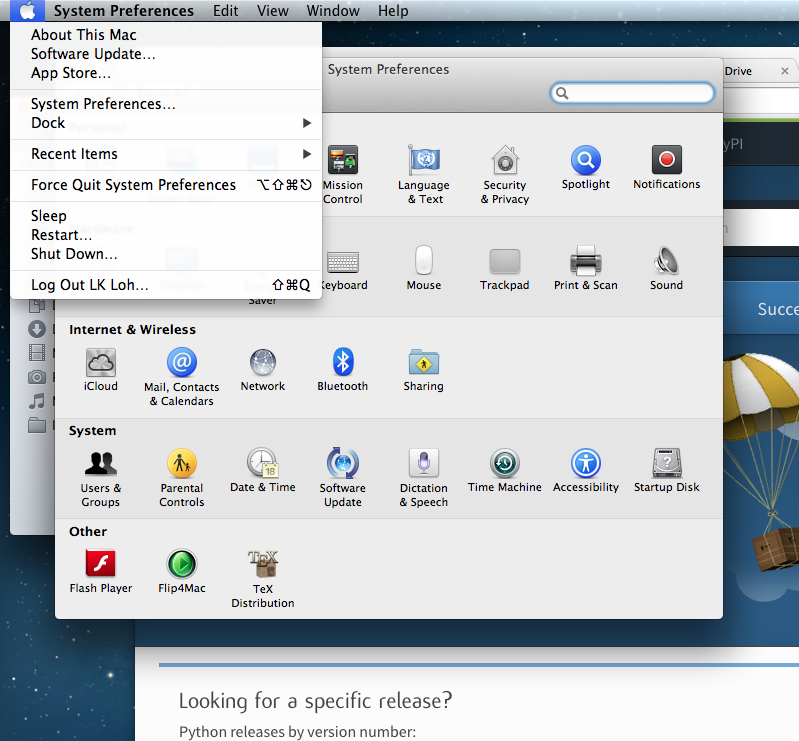
\includegraphics{system_preferences.png}


\section{Installing Python}
\label{docfiles/installing:installing-python}
\href{http://www1.i2r.a-star.edu.sg/~lins/codes/python.html}{Shaowei Lin} suggested Enthought Canopy to install all the Python packages easily. If you download the free version of Enthought Canopy, it gives you everything you need for installing AIMBAT properly. If you do not want to use Enthought Canopy, read the rest of this section to use Macports or Pip.


\section{Python Dependencies}
\label{docfiles/installing:python-dependencies}\begin{itemize}
\item {} 
\href{http://www.numpy.org/}{Numpy}

\item {} 
\href{http://www.scipy.org/}{Scipy}

\item {} 
\href{http://matplotlib.org/}{Matplotlib}

\item {} 
\href{http://ipython.org/}{iPython} (optional)

\end{itemize}


\chapter{Standing Order for Data (SOD)}
\label{docfiles/gettingData:standing-order-for-data-sod}\label{docfiles/gettingData::doc}

\section{Installing SOD}
\label{docfiles/gettingData:installing-sod}
First, download \href{http://www.seis.sc.edu/index.html}{SOD}.

Once you have gotten the folder for SOD, put it somewhere where you won't touch it too much. What I did was put the SOD folder in my home directory, though other places are acceptable as well, as long as its not too easy to delete it by accident.

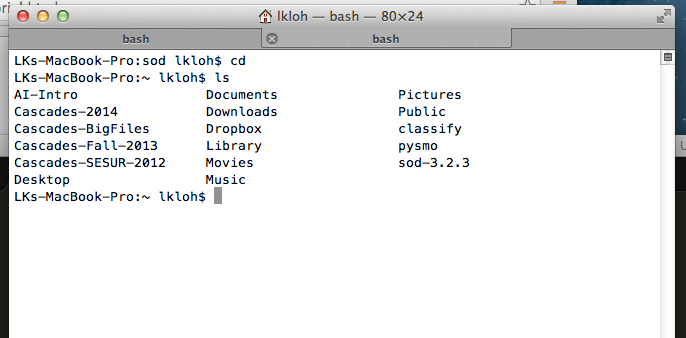
\includegraphics{sod_location.png}

Once you have it there, get the path to the sod folder's bin and put it in your path folder.

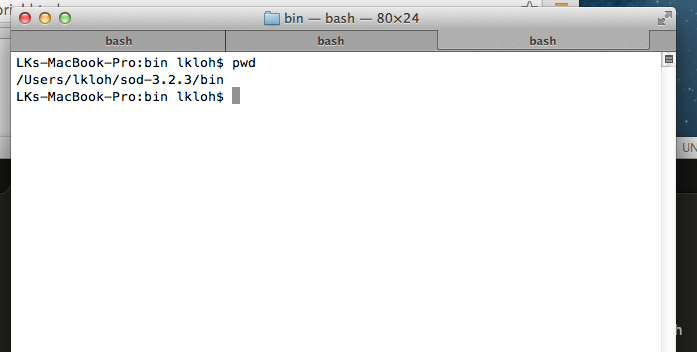
\includegraphics{path_to_sod_bin.png}

Inside my home directory's bash profile (you get the by typing \emph{cd}), you put the path to \emph{sod-3.2.3/bin} by adding in either the \emph{bash} or \emph{bash\_profile} or \emph{profile} files:


\section{Downloading Data with SOD}
\label{docfiles/gettingData:downloading-data-with-sod}\begin{quote}\begin{description}
\item[{Authors}] \leavevmode
\href{http://www.earth.northwestern.edu/~trevor/Welcome.html}{Trevor Bollmann}

\end{description}\end{quote}
\begin{enumerate}
\item {} \begin{description}
\item[{Create a sod recipe and place it in the folder that you would like the data to download to.}] \leavevmode\begin{itemize}
\item {} 
\emph{sod -f \textless{}recipename\textgreater{}.xml}

\end{itemize}

\end{description}

\item {} \begin{description}
\item[{Run verb''sodcut.sh'' to cut the seismogram around phase wanted}] \leavevmode\begin{itemize}
\item {} 
check model within \emph{cutevseis.sh}

\item {} 
run using \emph{sodcut.sh \textless{}name\textgreater{}}

\item {} 
watch sdir = processed seismograms

\item {} 
Run over the entire downloaded directory (the files sod downloaded)

\end{itemize}

\end{description}

\item {} \begin{description}
\item[{Run \emph{sodpkl.sh} (converts \emph{.sac} files to python pickles)}] \leavevmode\begin{itemize}
\item {} 
run using \emph{sodpkl.sh {[}options{]} \textless{}directory\textgreater{}}

\item {} 
output will automatically be zipped

\item {} 
run in DATA directory

\end{itemize}

\end{description}

\item {} \begin{description}
\item[{Run \emph{ttpick.py} (does travel time picking with plotting)}] \leavevmode\begin{itemize}
\item {} 
can use \emph{iccs.py} but it does not have plotting capabilities

\item {} 
run using \emph{ttpick.py {[}options{]} \textless{}pkl.gz file\textgreater{}}

\item {} 
do this one event at a time

\item {} 
use \emph{sacp2} to look at the stacking of the seismograms

\item {} 
you can sort the seismograms using the \emph{–s} flag

\end{itemize}

\end{description}

\item {} \begin{description}
\item[{run \emph{getsta.py} (creates a \emph{loc.sta} file)}] \leavevmode\begin{itemize}
\item {} 
\emph{getsta.py {[}options{]} \textless{}pkl.gz files\textgreater{}}

\end{itemize}

\end{description}

\item {} \begin{description}
\item[{Run EITHER of these:}] \leavevmode\begin{itemize}
\item {} 
FIRST CHOICE

\item {} 
run \emph{mccc2delay.py} (converts mccc delays to actual delays) by doing \emph{mccc2delay.py {[}option{]} \textless{}.mcp files\textgreater{}}

\item {} \begin{description}
\item[{run \emph{getdelay.py} (creates a delay file) by doing \emph{getdelay.py {[}options{]} \textless{}*.px\textgreater{}}}] \leavevmode\begin{itemize}
\item {} 
Can possibly use \emph{doplotsta.sh}, plots all of the events and their station delays

\end{itemize}

\end{description}

\item {} 
Run \emph{evmcdelay.sh}

\item {} \begin{description}
\item[{SECOND CHOICE}] \leavevmode\begin{itemize}
\item {} 
verb''ttcheck.py'' to compare the delay times of the p and s waves. Should form a nice cloud with the mean value in line with the cloud.

\end{itemize}

\end{description}

\end{itemize}

\end{description}

\item {} \begin{description}
\item[{If you need to remove a station from an event you can use verb''pklsel.py''}] \leavevmode\begin{itemize}
\item {} 
Run using verb''pklsel.py {[}pkl file{]} –d {[}stnm{]}'' to remove one station

\item {} 
Only works for one event at a time

\end{itemize}

\end{description}

\item {} \begin{description}
\item[{If you need to filter the data to be able to pick use verb''evsacbp.sh''}] \leavevmode\begin{itemize}
\item {} 
run using verb''evsacbp.sh {[}pkl file{]} bp1 bp2''

\item {} 
Automatically uses two corners

\item {} 
run in the whole downloaded directory (the one with the sac directory)

\end{itemize}

\end{description}

\end{enumerate}


\chapter{Analyzing Data}
\label{docfiles/analyzingData:analyzing-data}\label{docfiles/analyzingData::doc}

\section{Seismic Analysis Code (SAC)}
\label{docfiles/analyzingData:seismic-analysis-code-sac}
\href{http://www.iris.edu/files/sac-manual/}{SAC} is used.


\chapter{Picking Travel Times}
\label{docfiles/PickingTravelTimes:picking-travel-times}\label{docfiles/PickingTravelTimes::doc}
Hello, World! I love picking travel times manually!


\chapter{Citations}
\label{docfiles/citations:citations}\label{docfiles/citations::doc}

\chapter{Indices and tables}
\label{index:indices-and-tables}\begin{itemize}
\item {} 
\emph{genindex}

\item {} 
\emph{modindex}

\item {} 
\emph{search}

\end{itemize}

\begin{thebibliography}{VandecarCrosson1990-BulletinSeismologicalSocietyOfAmerica}
\bibitem[GoldsteinDodgeFirpo2003-InternationalGeophysics]{GoldsteinDodgeFirpo2003-InternationalGeophysics}{\phantomsection\label{docfiles/citations:goldsteindodgefirpo2003-internationalgeophysics} 
Goldstein, P., D. Dodge, M. Firpo, and L. Minner (2003), SAC2000: Signal processing and analysis tools for seismologists and engineers, International Geophysics, 81, 1613–1614.
}
\bibitem[Hunder2007-ComputingInScienceAndEngineering]{Hunder2007-ComputingInScienceAndEngineering}{\phantomsection\label{docfiles/citations:hunder2007-computinginscienceandengineering} 
Hunter, J. (2007), Matplotlib: A 2D Graphics Environment, Computing in Science \& Engi- neering, 3(9), 90–95.
}
\bibitem[LouVanderleeLloyd2013-SeismologicalResearchLetters]{LouVanderleeLloyd2013-SeismologicalResearchLetters}{\phantomsection\label{docfiles/citations:louvanderleelloyd2013-seismologicalresearchletters} 
AIMBAT: A Python/Matplotlib Tool for Measuring Teleseismic Arrival Times. Xiaoting Lou, Suzan van der Lee, and Simon Lloyd (2013), Seismol. Res. Lett., 84(1), 85-93, doi:10.1785/0220120033.
}
\bibitem[VandecarCrosson1990-BulletinSeismologicalSocietyOfAmerica]{VandecarCrosson1990-BulletinSeismologicalSocietyOfAmerica}{\phantomsection\label{docfiles/citations:vandecarcrosson1990-bulletinseismologicalsocietyofamerica} 
VanDecar, J. C., and R. S. Crosson (1990), Determination of teleseismic relative phase arrival times using multi-channel cross-correlation and least squares, Bulletin of the Seismological Society of America, 80(1), 150–169.
}
\end{thebibliography}



\renewcommand{\indexname}{Index}
\printindex
\end{document}
